\section{Results}

\subsection{Environmental conditions}

\begin{figure}[here]
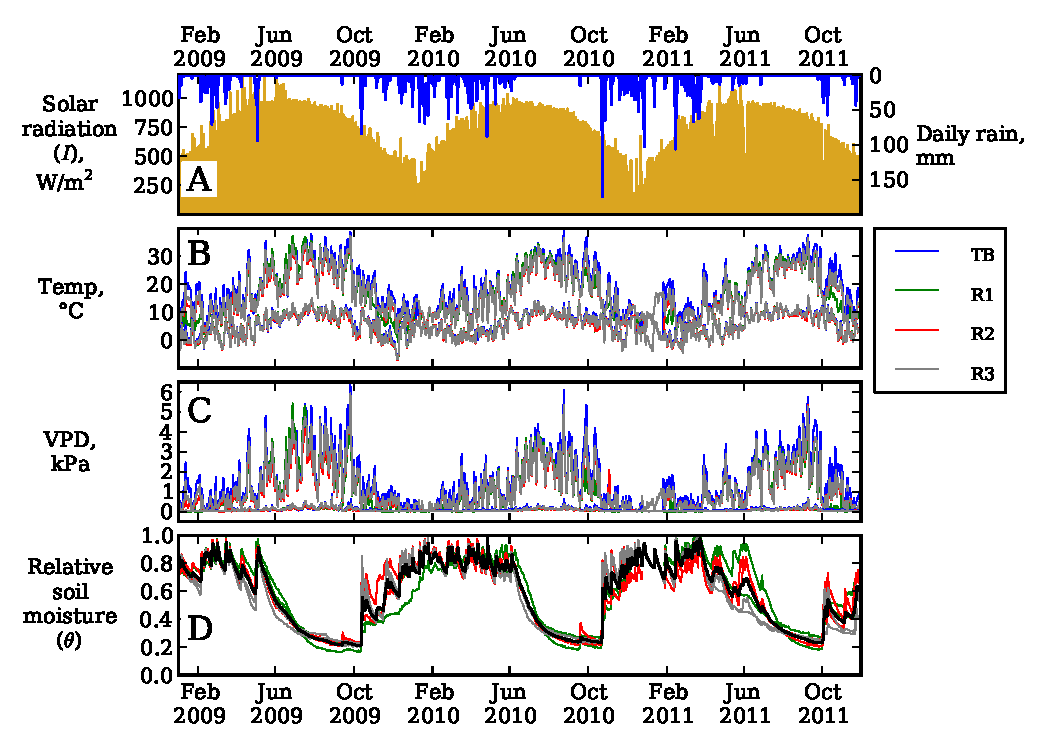
\includegraphics[width=0.9\textwidth]{ch1-sapflow/figures/Figure03.pdf}
\caption{Climatic and hydrologic time series: (a) solar radiation (\textit{I}, yellow) and daily rainfall (blue), both measured unobstructed in an open field; (b) daily minimum and maximum air temperature (\textit{T}) at ground stations (R1, R2, R3) and canopy station (TB); (c) daily minimum and maximum vapor pressure deficit (\textit{VPD}) at ground stations (R1, R2, R3) and canopy station (TB); (d) red, green, and gray: daily average relative soil moisture (\textit{$\theta$}), averaged over each of the 6 profiles shown in Figure \ref{fig:sapflow_map} (colors indicate the profile's nearest weather station, as in panel (b) legend); black: average of the 6 profile averages of relative soil moisture.}
\label{fig:sapflow_met}
\end{figure}

The ACRR has a Mediterranean climate with a marked winter wet season and summer dry season.  The wet season at the ACRR extends from approximately October through April (90\% of the annual precipitation fell in these months in 2009-2011), and very little rain falls during July through September (less than 1\% in 2009-2011; Figure \ref{fig:sapflow_met}(a)).  Clear sky \textit{I} is maximum in late June (summer solstice) and minimum in late December (winter solstice), and \textit{I} can be reduced by 50 to 90\% on cloudy days.  The annual cycle of \textit{T} lags behind that of \textit{I}, with a peak in July and August and a minimum in January or February. The mean July-September \textit{T} for 2009-2011 was 18$^{\circ}$C, and the mean December-February \textit{T} was 5$^{\circ}$C (weather station R3).  The annual cycle of \textit{VPD} follows that of \textit{T} and also peaks in July or August.  \textit{T} and \textit{RH} vary somewhat along the hillslope: on clear days, the air is warmer and drier in the upper canopy and upslope, and the air is cooler and more humid downslope (up to 10$^{\circ}$C cooler at downslope ground level than in the canopy at midday in winter; Figure \ref{fig:sapflow_met}(b) and (c)).  Mean annual \textit{P} in the vicinity of the ACRR (National Climatic Data Center GHCN precipitation station USC00048490, 18 km NNE of the ACRR; data from 1960-2000; \cite{williams2012modifications}) is 1800 mm, with significant interannual variability (standard deviation of 500 mm); on average, 3\% ($\pm$3\% standard deviation) of annual precipitation falls in July through September.  During the study period, precipitation at Rivendell ranged between a minimum of 1500 mm in water year 2008-2009 and a maximum of 2100 mm in water year 2010-2011.

Water storage below ground is also highly seasonal. The water table, measured by 12 on-site wells, remains near 5 m below ground throughout the year at downslope wells, but upslope it ranges from $\sim$10 m below ground in the wet season to $\sim$20 m below ground in the dry season.   Soil moisture ($\theta$) is high and dynamic during the winter rainy season but dries to fairly steady and very low values during the summer dry season (Figure \ref{fig:sapflow_met}(d); \cite{salve2012rain}).  

\subsection{Sap velocities}

\begin{figure}[here]
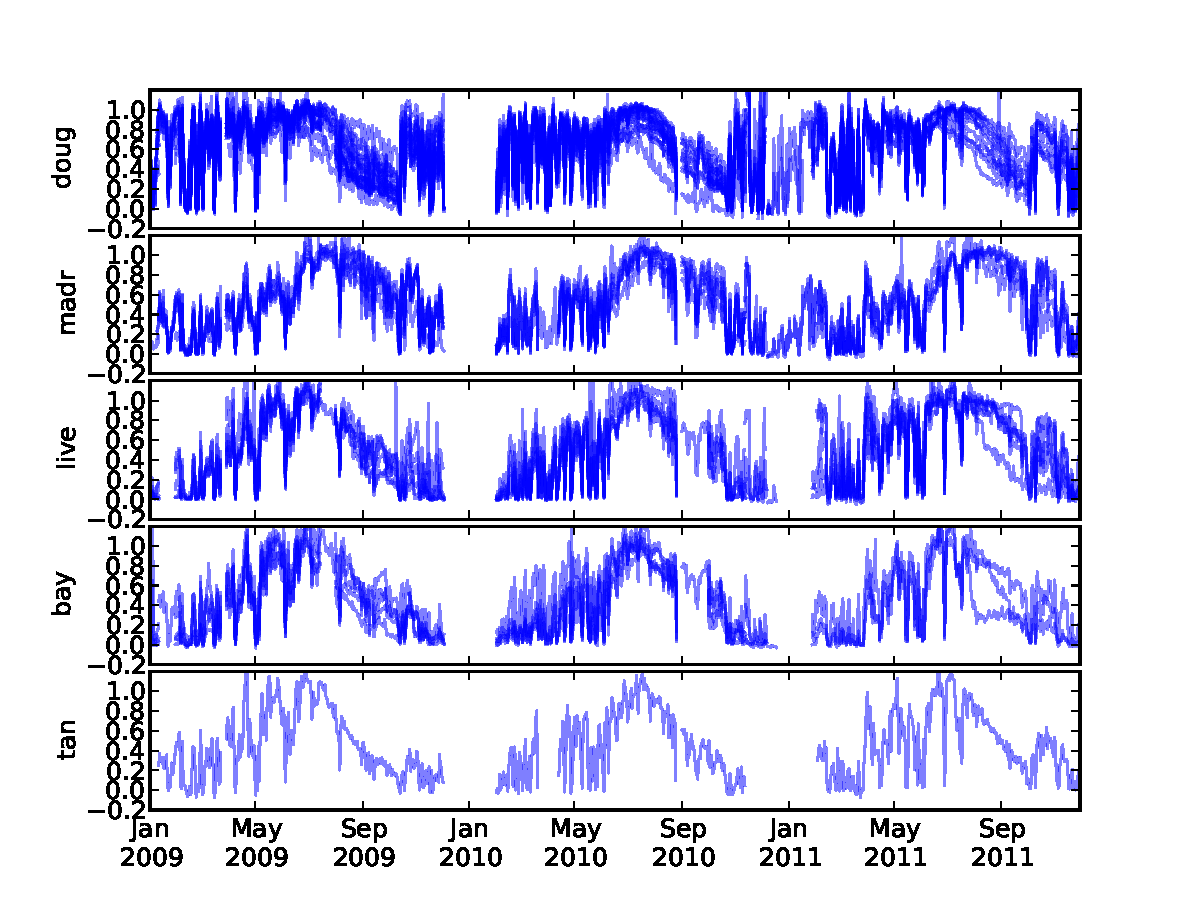
\includegraphics[width=0.9\textwidth]{ch1-sapflow/figures/Figure04.pdf}
\caption{Daily maximum normalized sap velocities for each sensor, separated by species.  Each sensor's line is slightly transparent, so that overlapping lines create darker blue colors.  Data gaps are due largely to power failure during times of low insolation.  Species codes: doug=Douglas-fir; madr=Pacific madrone; live=interior live oak; tan=tanoak.}
\label{fig:sapflow_normvel}
\end{figure}

The 99.5th percentile velocities for each sensor and each stage are listed in Table \ref{tbl:tree_props}, and the timeseries of daily maximum normalized instantaneous velocity for each sensor are shown in Figure \ref{fig:sapflow_normvel}, separated by species (only the daily maximum is shown for visibility.)  For the following analyses, we constructed tree-averaged timeseries for trees with multiple sensors by averaging the normalized velocities at each measurement time for all sensors in a given tree.  This tree-averaging was performed because sensors within a tree covaried strongly for all trees (Table \ref{tbl:sapflow_covar}), and thus sensors in the same tree were not independent.

\begin{table}
  \caption{Covariation of sap velocities within the same tree.}
  \label{tbl:sapflow_covar}
  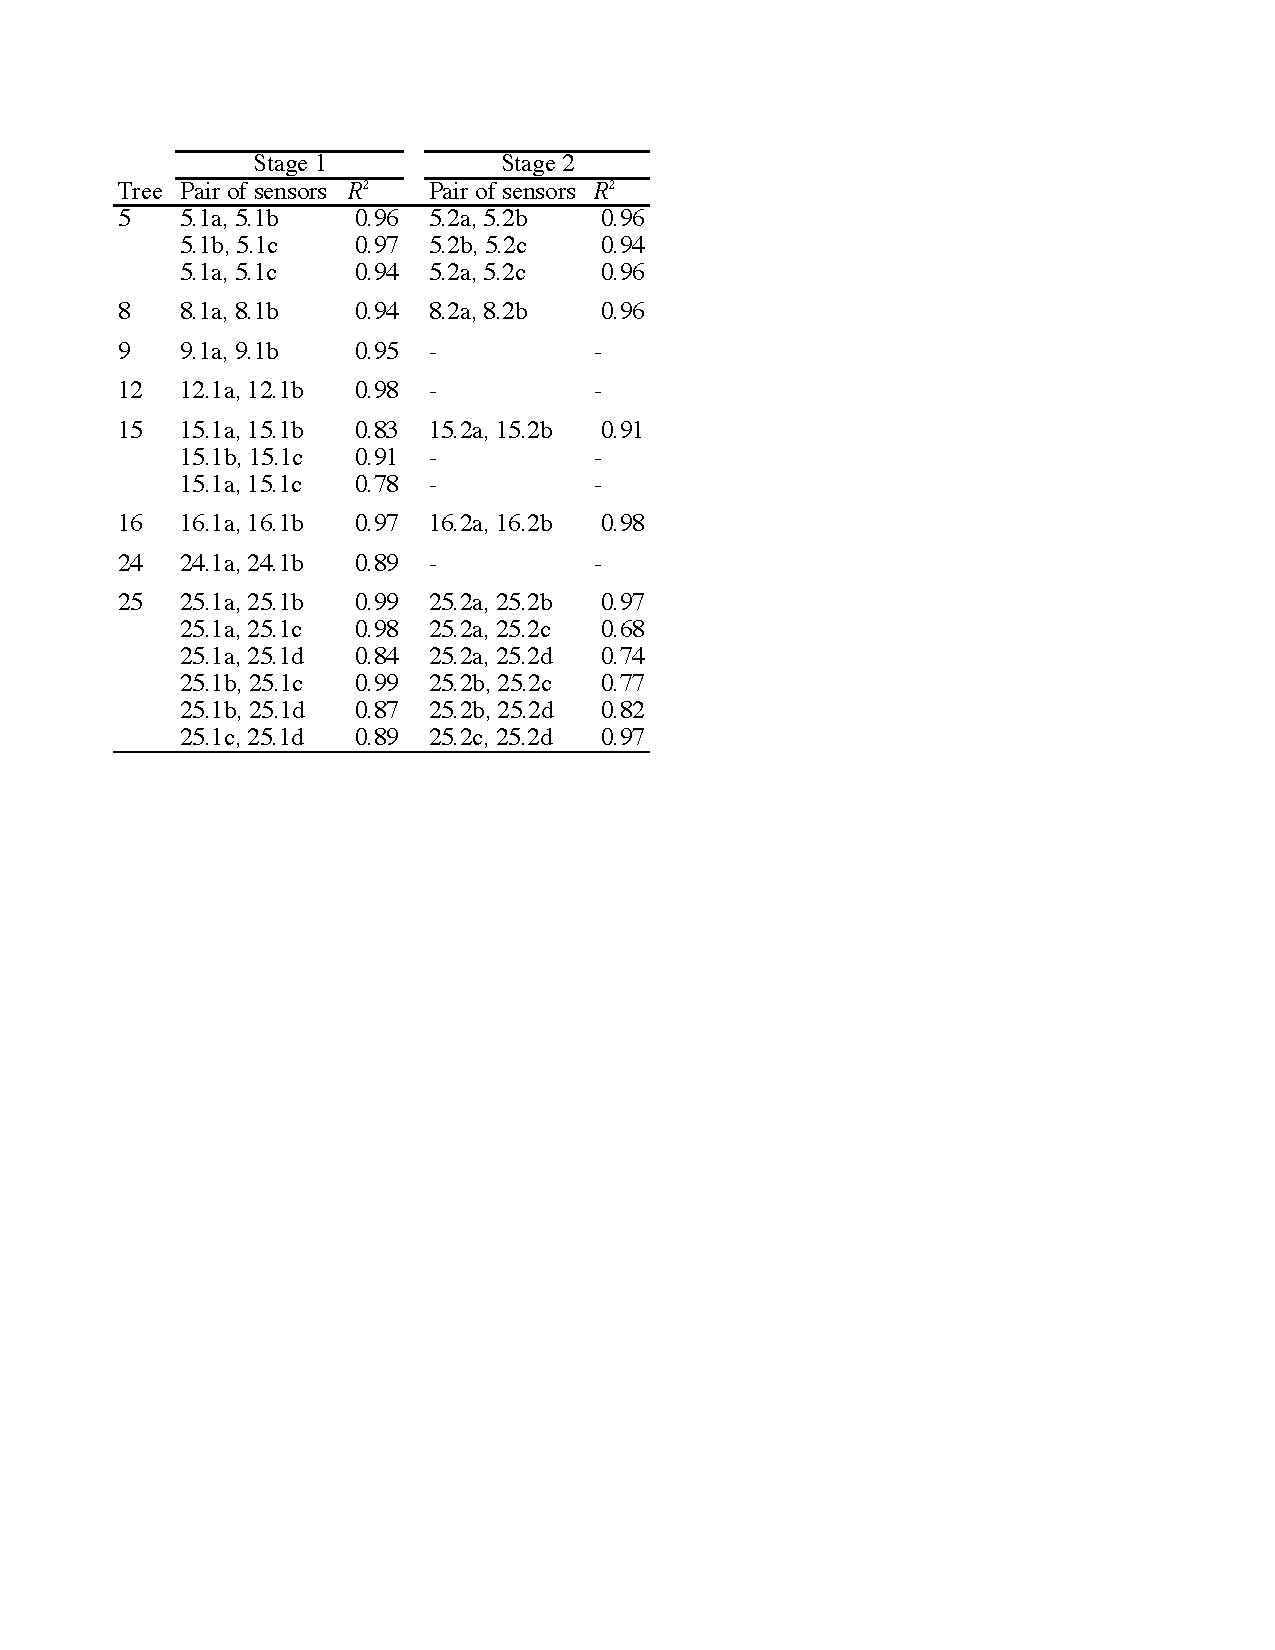
\includegraphics[width=\linewidth]{ch1-sapflow/tables/TableA1.pdf}
\end{table}

\subsection{Seasonal patterns: Principal Component Analysis}
\label{sec:seasonal}

\begin{figure}[here]
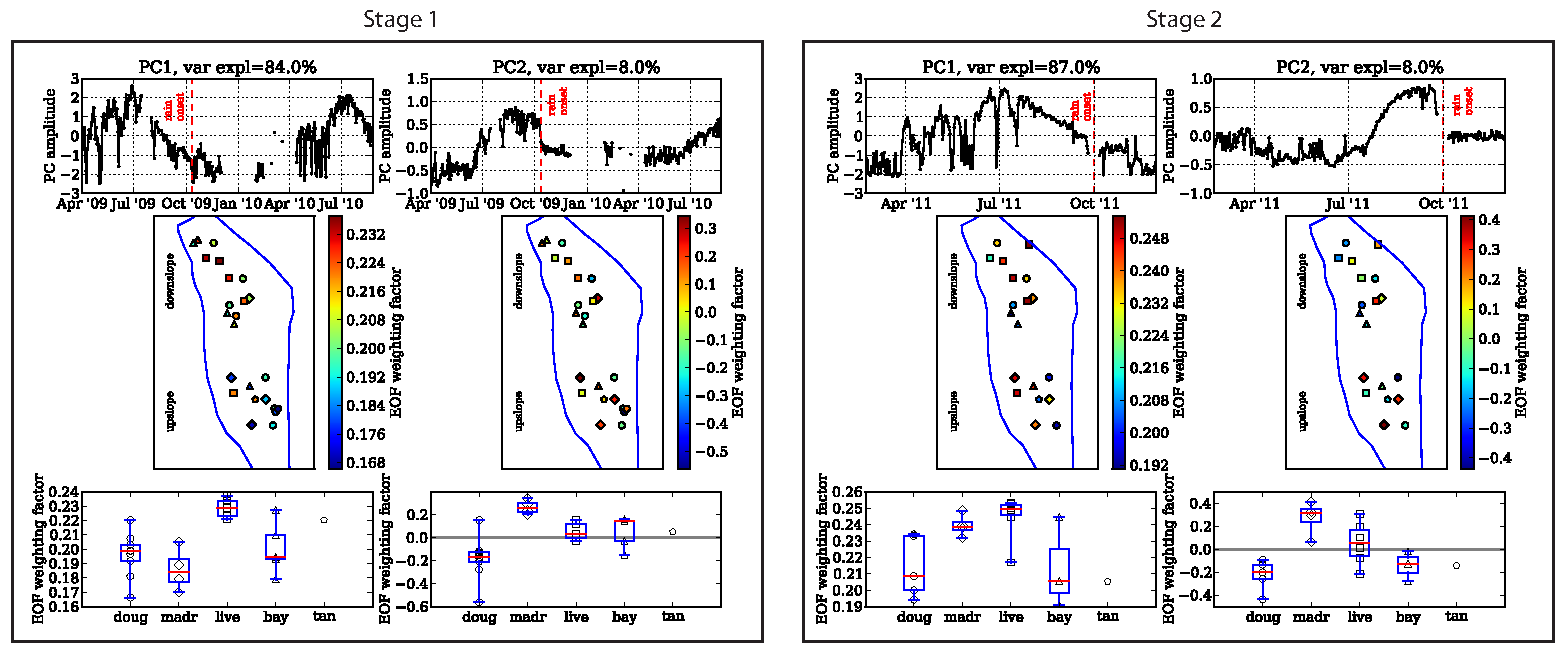
\includegraphics[width=0.9\textwidth]{ch1-sapflow/figures/Figure05.pdf}
\caption{PCA results for all sensors, for stage 1 (left box) and stage 2 (right box).  Within each stage, left column: PC/EOF 1, right column: PC/EOF 2.  Top row: principal component time patterns.  Circles show days included in the analysis.  Gaps represent periods of missing data longer than 4 days.  Middle row: maps of EOF weighting factors for all trees included in the analysis.  Symbol shape indicates species, as in Figure \ref{fig:sapflow_map}.  Bottom row: EOF weighting factors, sorted by species.  Box plot divides the quartiles of the distribution; red line shows the median.  Both the PCs and EOFs are unitless, because the analysis used normalized velocities.}
\label{fig:sapflow_eof}
\end{figure}

The time pattern that explains the most variance among all sap flow sensors, PC1, represents the common annual cycle, with a peak in early July and lower values through the winter, mirroring the annual cycle of solar radiation (Figure \ref{fig:sapflow_eof}, left column in each stage).  PC1 also contains the abrupt drops in sap flow on rainy days in winter and spring, when almost all sensors have very low sap velocity.  The annual cycle pattern is evident in PC1 for both stages, and PC1 explains 84\% of the variance in stage 1 (2009-2010) and 87\% of the variance in stage 2 (2011).  All sensors in both stages have positive weighting factors for PC1, meaning that all sensors display a component of this annual cycle pattern.  In stage 1, downslope trees tend to resemble PC1 more strongly than do upslope trees (i.e., have larger positive weighting factors).

The time pattern that explains the next-largest fraction of the variance, PC2, acts as a phase offset from the PC1 annual cycle, with a positive peak in the July-October dry season and negative values for the rest of the year (Figure \ref{fig:sapflow_eof}, right column in each stage).  Again, the PC2 pattern is similar between the two stages of deployment.  A positive EOF2 weighting factor for PC2 indicates greater July-October transpiration than PC1 and less November-June transpiration, and thus a shift in the peak season of transpiration later into the dry season.  On the other hand, a negative EOF2 weighting factor indicates less July-October transpiration compared to PC1 and greater transpiration in the rest of the year, and thus indicates a shift in peak transpiration earlier toward the wet spring.  PC2 explains 8\% of the variance in both stages.

The direction of the transpiration phase shift is species-specific.  Pacific madrones have the most positive weighting factors for PC2 in both stages, indicating a phase shift of peak transpiration later into the dry season (Figure \ref{fig:sapflow_eof}, bottom right panel in each stage).  Douglas-firs, in contrast, almost all have negative values, indicating a phase shift earlier toward the wet spring season.  Live oaks, bays, and the tanoak have weighting factors closer to zero, indicating less phase shift away from the PC1 pattern.

Additionally, the PC2 time pattern shows an abrupt decrease at the onset of the rainy season in October of each year.  Thus, Pacific madrone sap velocities, with positive PC2 amplitudes, decrease sharply at the onset of the rainy season, while Douglas-fir velocities, with negative PC2 amplitudes, increase sharply.

\subsection{Sensitivities to environmental drivers}
\label{sec:envresponse}

These PC/EOF patterns are empirical, indicating the dominant patterns of variability and demonstrating that there is a seasonal offset of transpiration between evergreen tree species at this site.  In order to investigate the drivers of this difference, we quantify the response of sap velocity to environmental variables.

\begin{figure}[here]
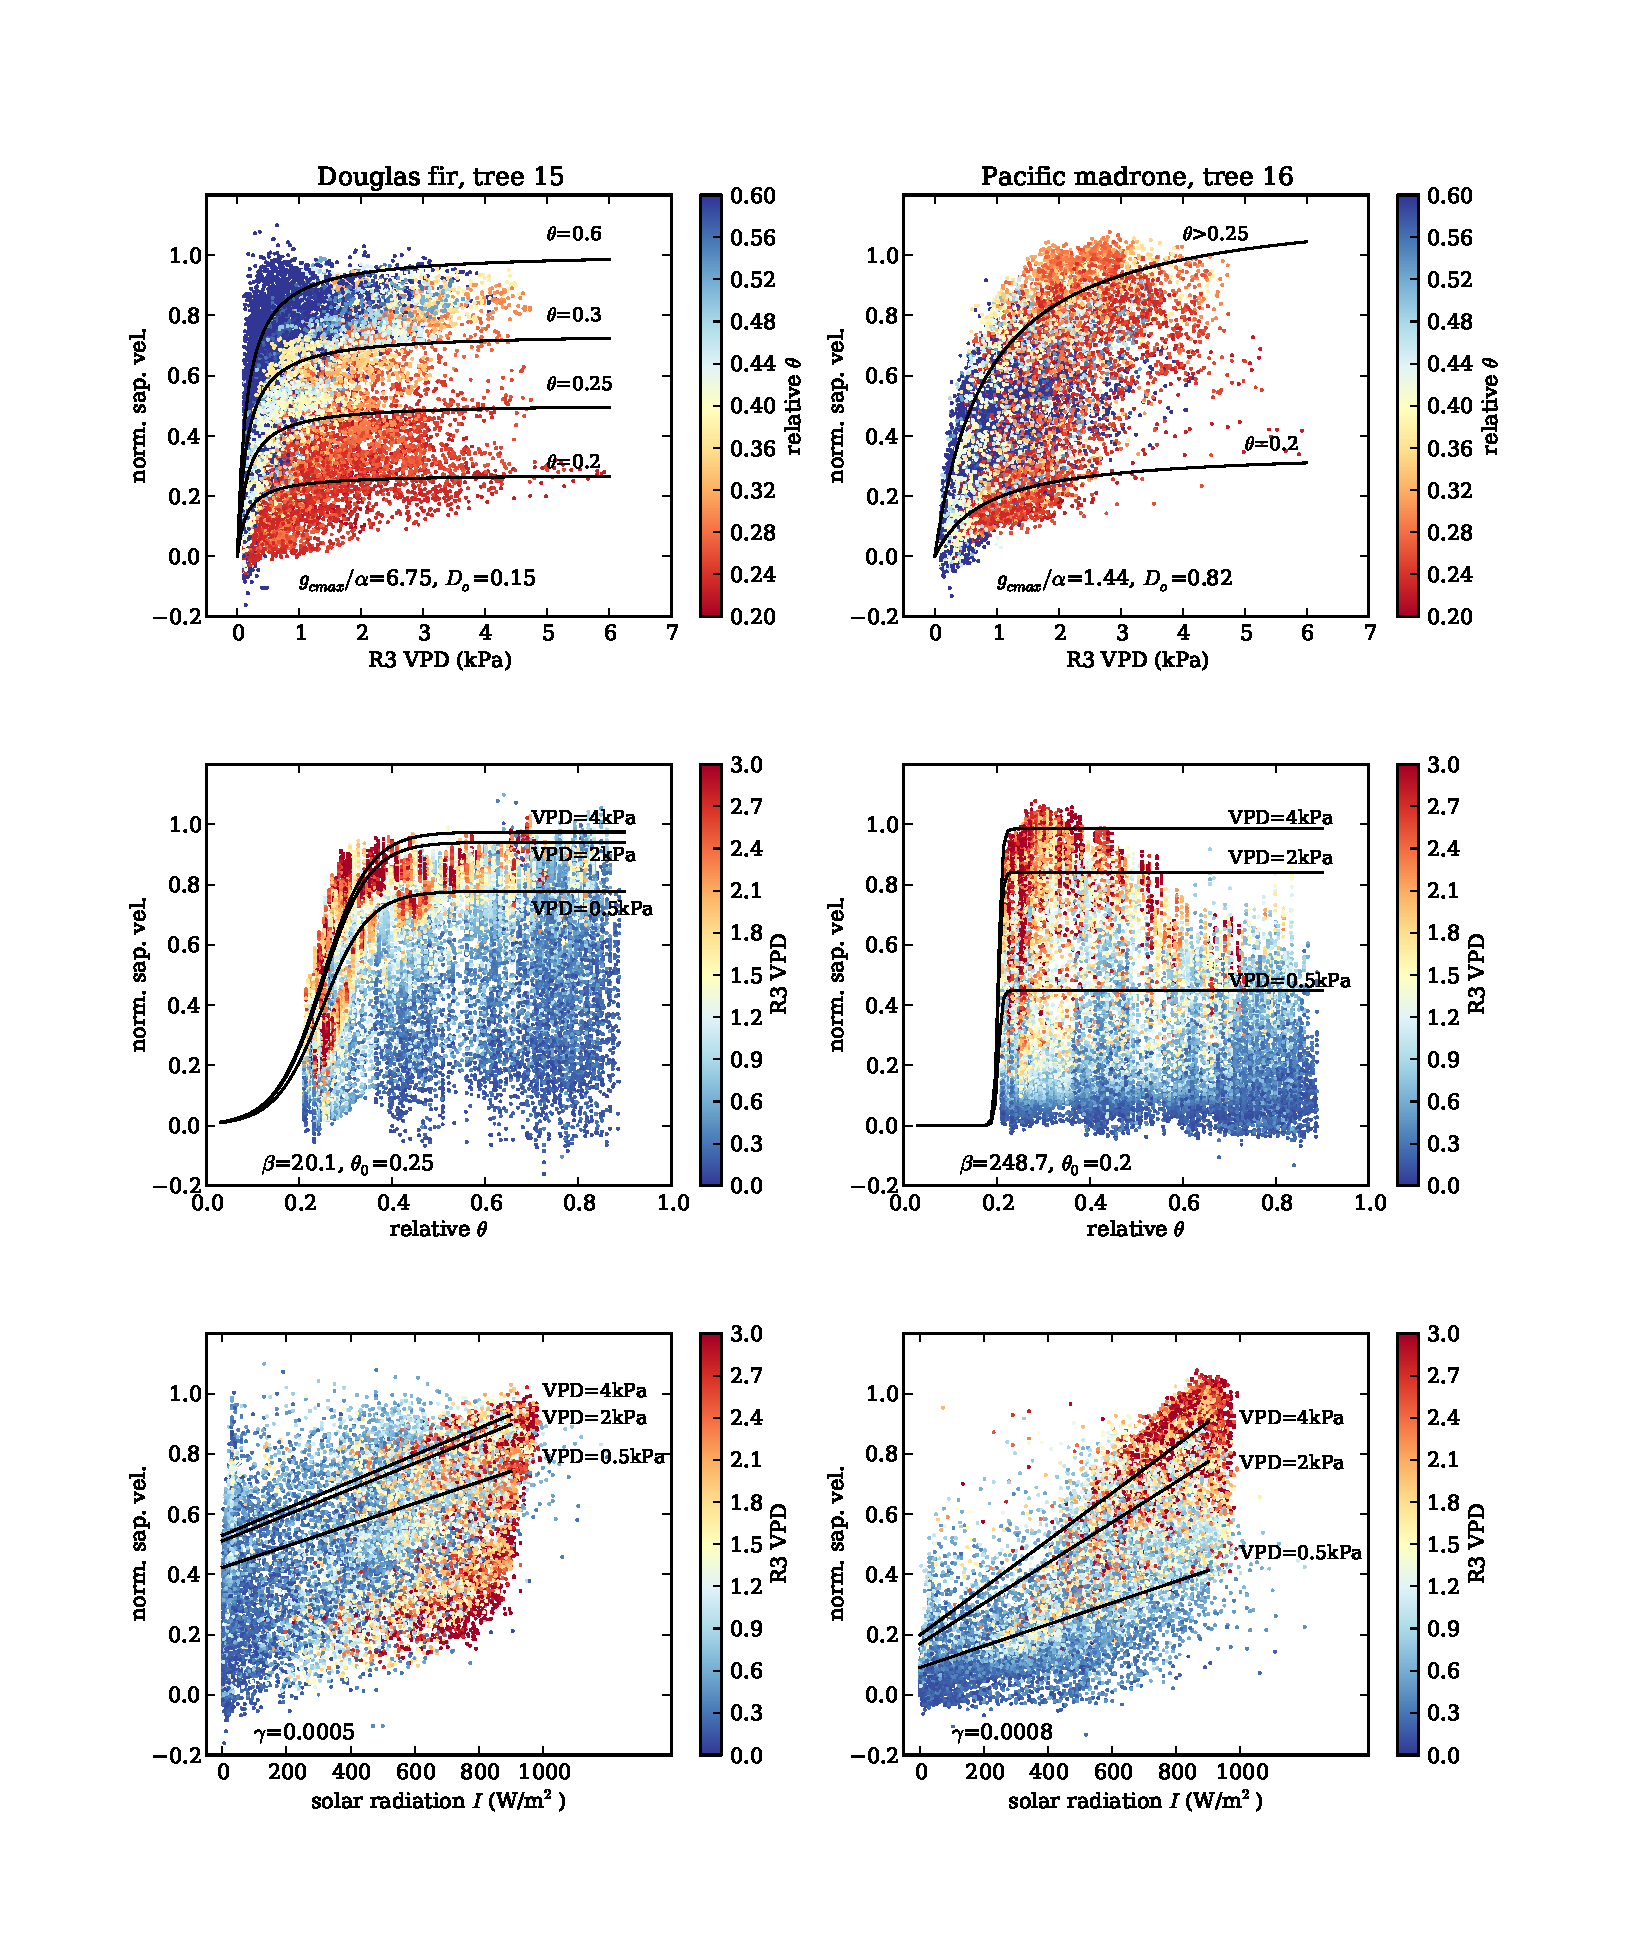
\includegraphics[width=0.9\textwidth]{ch1-sapflow/figures/Figure06.pdf}
\caption{Sap flow response to environmental drivers for example trees.  Left column: tree 15, Douglas fir.  Right column: tree 16, Pacific madrone.  Top row: \textit{VPD} versus normalized instantaneous sap velocity, with symbols colored by site-averaged relative $\theta$.  Lines show the fitted \textit{VPD} function with different cases of soil moisture.  Middle row: site-averaged site-averaged relative $\theta$ versus normalized instantaneous sap velocity, with symbols colored by \textit{VPD}.  Lines show the fitted soil moisture function with different cases of \textit{VPD}.  Bottom row: solar radiation \textit{I} at station AM versus normalized instantaneous sap velocity, with symbols colored by \textit{VPD}.  Lines show the fitted radiation function, with different cases of \textit{VPD}.}
\label{fig:sapflow_scatter}
\end{figure}

Two end-member cases of tree transpiration response to \textit{VPD}, $\theta$, and \textit{I} are shown in Figure \ref{fig:sapflow_scatter}, with Douglas-fir tree 15 in the left column and Pacific madrone tree 16 in the right column.  In the Douglas-fir, sap flow increases sharply with increasing \textit{VPD} at low \textit{VPD} and then plateaus at higher \textit{VPD}; the low value of $D_o$ captures this behavior.  In contrast, the Pacific madrone's sap flow increases more gradually with increasing \textit{VPD}, and the higher value of $D_o$ quantifies this behavior.

The Douglas-fir's higher value of $\theta_o$ shows that this Douglas-fir's sap flow begins to decline at higher values of $\theta$.  The lower value of $\theta_o$ for the Pacific madrone reflects that the Pacific madrone's sap flow does not decline until lower values of $\theta$.  The parameter $\beta$ represents how fast sap flow declines in response to soil moisture limitation, once the decline starts.  Higher $\beta$ (as with the Pacific madrone in Figure \ref{fig:sapflow_scatter}) means a more rapid decline below the threshold, and lower $\beta$ (as with the Douglas-fir in Figure \ref{fig:sapflow_scatter}) means a more gradual decline.

The response of sap velocity to \textit{I} is captured by the slope $\gamma$, which describes how quickly the sap flow increases with increasing \textit{I}.  In Figure \ref{fig:sapflow_scatter}, the Douglas-fir has a low slope, meaning its sap flow remains high at low \textit{I} and increases only slightly with increasing \textit{I}; while the Pacific madrone has a higher positive slope, meaning that it has low sap flow at low \textit{I} and increases more strongly with increasing \textit{I}.

\begin{figure}[here]
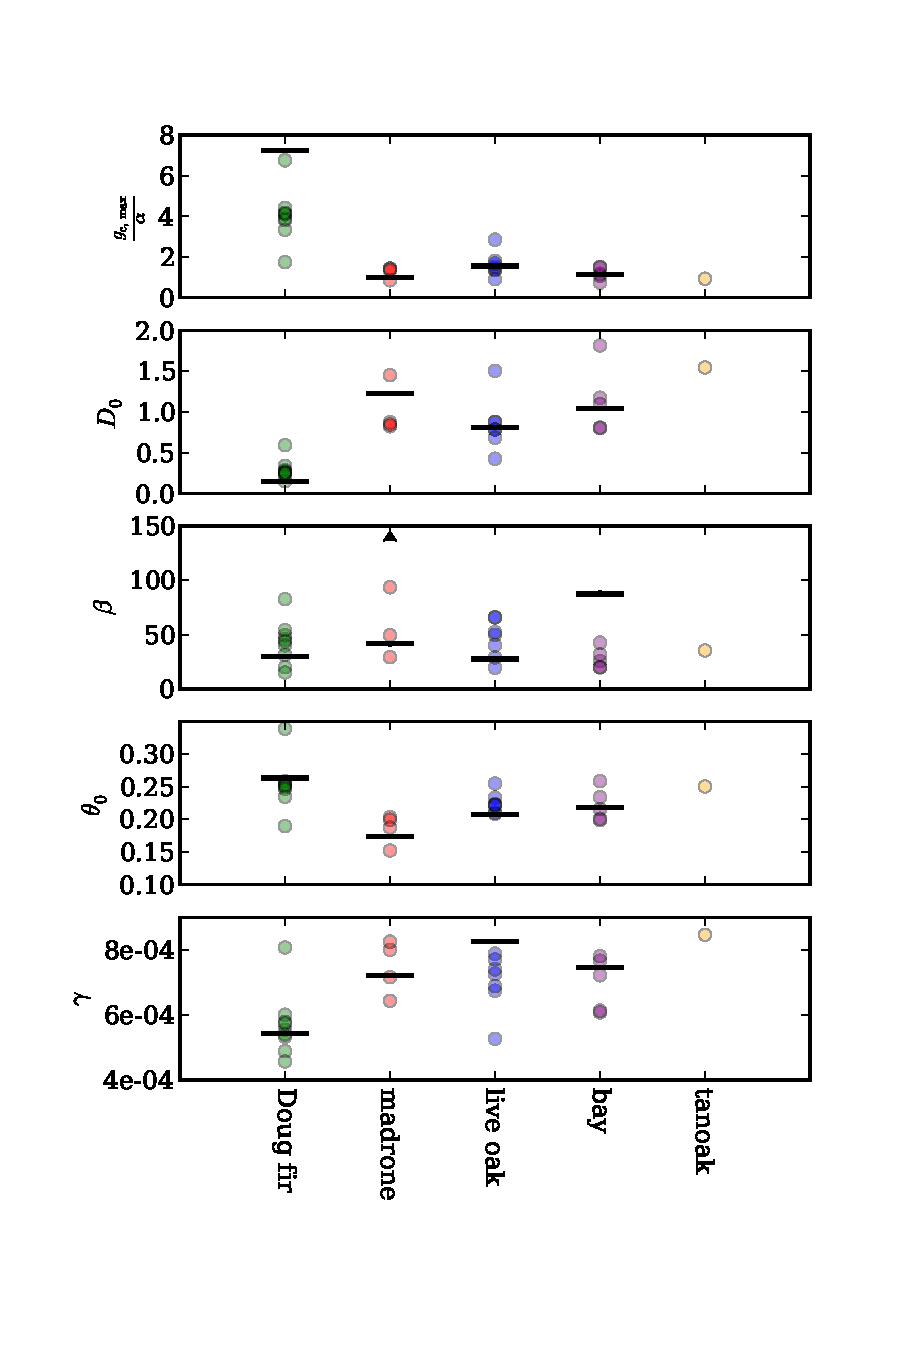
\includegraphics[width=0.65\textwidth]{ch1-sapflow/figures/Figure07.pdf}
\caption{Estimated Jarvis parameters, sorted by species.  Each circle represents the median of the posterior distribution for an individual sensor.  Black horizontal lines show the medians of the posterior distributions for the species-averaged timeseries parameters; vertical black error bars show the 95\% HPD interval (for most species-averaged timeseries parameters, this interval is smaller than the thickness of the horizontal line.)  Row 1: $g_{cmax}/\alpha$ parameter (kPa$^{-1}$), indicating sap velocity at low values of \textit{VPD} and radiation.  Row 2: $D_o$ parameter (kPa), which measures the curvature of the sap velocity increase with increasing \textit{VPD}.  Row 3: $\beta$ parameter (unitless), which measures the rate of sap flow decline around a soil moisture threshold.  The black triangle indicates that one madrone tree has a $\beta$ value higher than 150. Row 4: $\theta_0$ parameter (unitless), which measures the soil moisture value at which sap flow decline is centered.  Row 5: $\gamma$ parameter ((W/m$^2$)$^{-1}$), slope of the sap velocity increase with increasing radiation.}
\label{fig:sapflow_params}
\end{figure}

The Jarvis model parameters for all trees, separated by species, are shown in Figure \ref{fig:sapflow_params} and summarized in Table \ref{tbl:sapflow_mcmc}.  For 25 of the 26 trees, the posterior distributions of all five parameters are sharply peaked and well within the initial uniform prior chosen (example posterior distributions are shown in Figure \ref{fig:sapflow_posterior}).  One Pacific madrone tree (tree 16) has a broader distribution for $\beta$ than other trees (see 95\% HPD interval in Table \ref{tbl:sapflow_mcmc}.)

\begin{table}
  \caption{Median values of estimated Jarvis parameter distributions for each tree, with uncertainties calculated from the 
95\% HPD interval.}
  \label{tbl:sapflow_mcmc}
  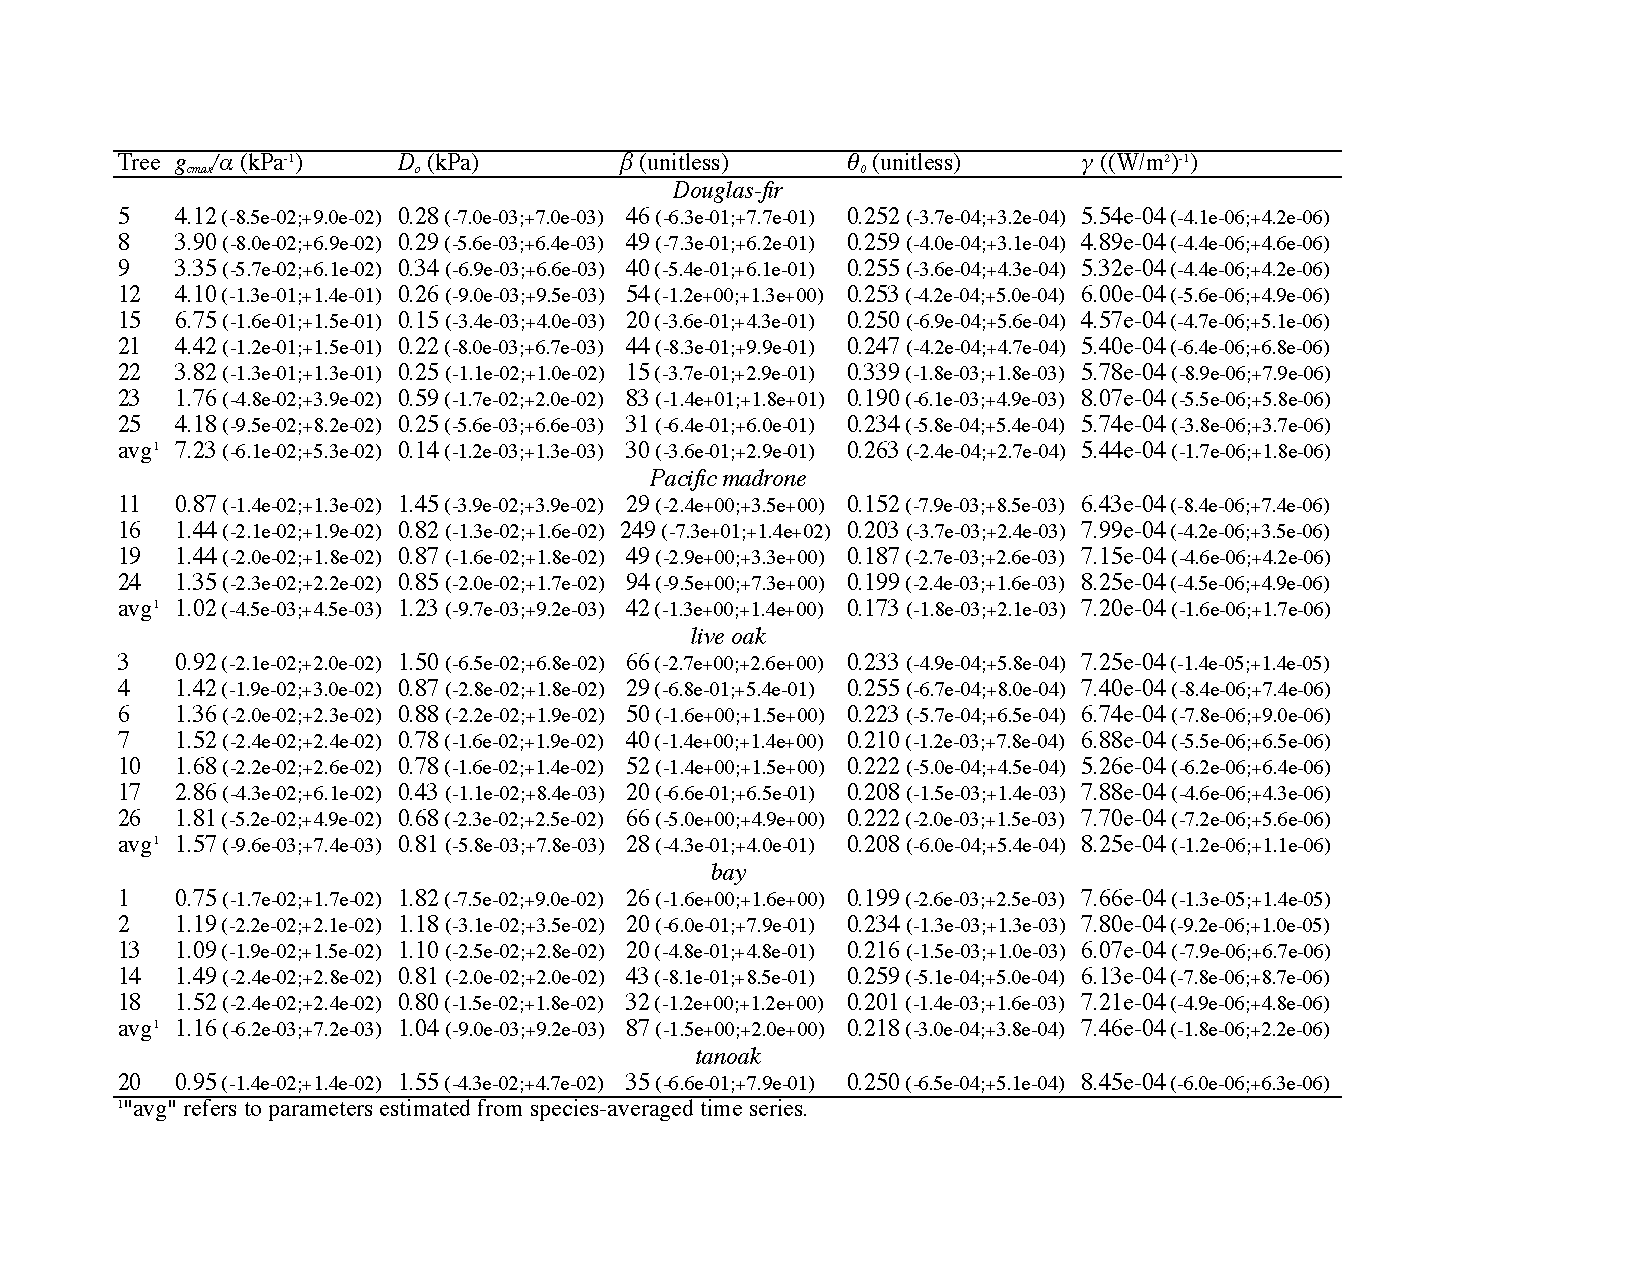
\includegraphics[width=\linewidth]{ch1-sapflow/tables/TableA2_cropped.pdf}
\end{table}

\begin{figure}[here]
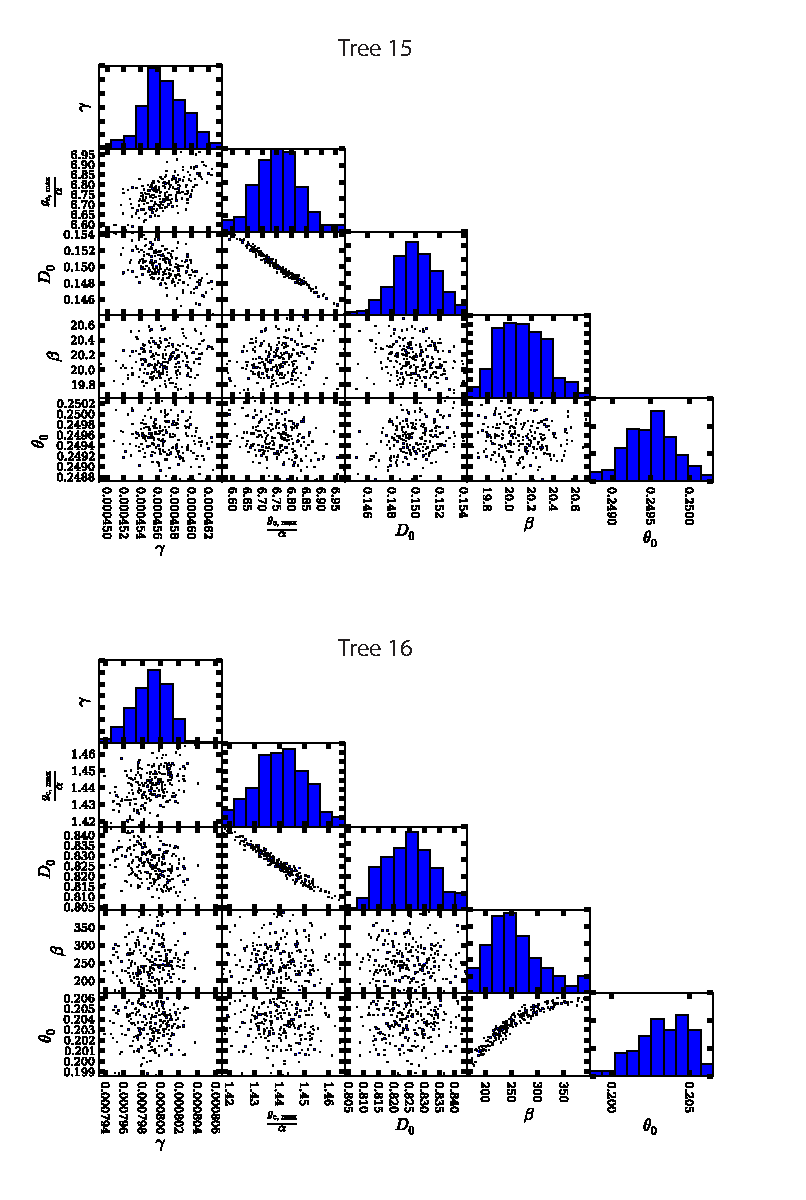
\includegraphics[width=0.75\textwidth]{ch1-sapflow/figures/FigureA1.pdf}
\caption{Panels on the diagonal: posterior distributions of environmental response parameters for the example Douglas-fir sensor (top) and the example Pacific madrone sensor (bottom.)  Panels below the diagonal: covariation of each pair of parameters for each example sensor.}
\label{fig:sapflow_posterior}
\end{figure}

The distributions of the median \textit{VPD} parameters for all sensors and for the species-averaged timeseries parameters ($g_{cmax}/\alpha$ and $D_o$, Figure \ref{fig:sapflow_params}, rows 1 and 2) confirm that sap flow in Douglas-firs across this site increases quickly at low \textit{VPD} and plateaus at high \textit{VPD} (high $g_{cmax}/\alpha$ and low $D_o$).  The broadleaf species, in contrast, respond more gradually with increasing \textit{VPD} (lower $g_{cmax}/\alpha$ and higher $D_o$).

The fitted soil moisture parameter $\theta_o$ (Figure \ref{fig:sapflow_params}, row 4) also shows a species difference.  Douglas-firs have higher $\theta_o$ values; their decline in response to soil moisture limitation is centered on a relative $\theta$ value of 0.263 (from species-averaged timeseries;  $-2.4 \times 10^{-4}$, $+2.7 \times 10^{-4}$ 95\% HPD interval).  Pacific madrones, on the other hand, have lower $\theta_o$ values when fitted to the sigmoid functional form, with declines centered on 0.173 (from species-averaged timeseries; $-1.8 \times 10^{-3}$, $+2.1 \times 10^{-3}$ 95\% HPD interval).

The parameter $\beta$ for individual sensors is more evenly distributed across species, indicating little species difference in the rate of sap flow decline below each individual tree's soil moisture threshold (Figure \ref{fig:sapflow_params}, row 3).  Pacific madrone sensors tend to have higher values of $\beta$, indicating that once their low $\theta_o$ is reached, their transpiration declines sharply; however, $\theta$ values below the Pacific madrone $\theta_o$ values were infrequently observed, so their decline is not well constrained.

The slopes $\gamma$ of the radiation function (Figure \ref{fig:sapflow_params}, row 5) range from $5 \times 10^{-4}$ to $8 \times 10^{-4}$ (W/m$^2$)$^{-1}$.  Douglas-firs tend to have lower slopes, indicating relatively high sap velocity at low \textit{I} and less sensitivity to \textit{I} increase.  In contrast, the broadleaf species (Pacific madrones, live oaks, and bays) have higher slopes, indicating that their sap velocity increases more with increasing \textit{I}.

In general, the parameters do not vary systematically by tree diameter or position on the slope.  There is some increase of $g_{cmax}/\alpha$ and decrease of $D_o$ with increasing tree diameter, but this effect is difficult to disentangle from species differences, because all trees larger than 60 cm in diameter are Douglas-firs, while many of the smaller trees are broadleaf species.  This lack of diameter- and position-dependence is consistent with the PCA results, which suggest that species differences represent the largest contribution to the observed sap flow variability.

The MCMC results show that Douglas-firs and Pacific madrones are at opposite ends of the spectrum of response to \textit{VPD} and $\theta$.  Douglas-firs increase sharply in response to \textit{VPD} and then plateau, while Pacific madrones increase gradually and continually with increasing \textit{VPD}.  Douglas-firs decline significantly at low $\theta$ values, while Pacific madrones show little to no suppression with low $\theta$ values.  Live oaks and bays fall between these end-member responses.

\subsection{Synoptic-scale temporal variability}

\begin{figure}[here]
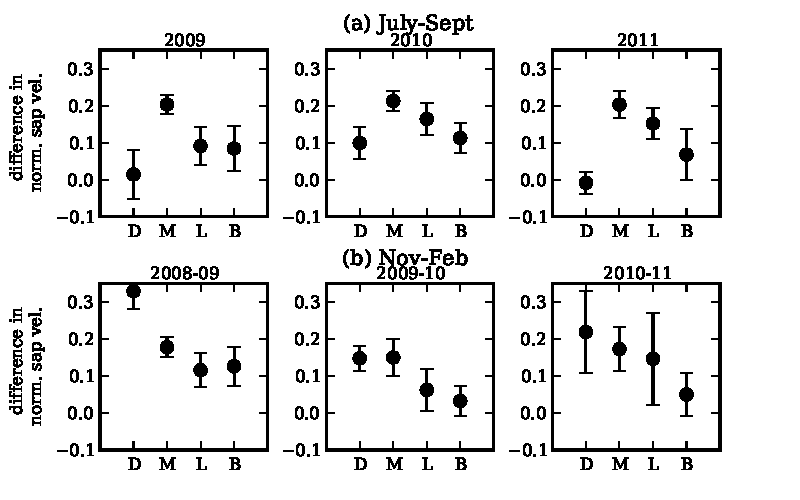
\includegraphics[width=0.9\textwidth]{ch1-sapflow/figures/Figure08.pdf}
\caption{Difference in normalized daily integral sap velocity between high \textit{VPD} days and low \textit{VPD} days, by species (D=Douglas fir, M=Pacific madrone, L=live oak, B=bay).  Circles show mean difference across all trees in the species for that season, and error bars show one standard deviation.  Row (a): July to September, where high \textit{VPD} days are days with maximum \textit{VPD}$>$2 kPa, and low \textit{VPD} days are days with maximum \textit{VPD}$<$2 kPa.  Row (b): November to February, where high \textit{VPD} days are days with maximum \textit{VPD}$>$0.5 kPa, and low \textit{VPD} days are days with maximum \textit{VPD}$<$0.5 kPa.}
\label{fig:sapflow_synoptic}
\end{figure}

The different sensitivity to \textit{VPD} in Douglas-firs and Pacific madrones translates to different transpiration response to synoptic-scale (daily to weekly, weather-scale) variability in atmospheric evaporative demand.  In the summer dry season, \textit{VPD} varies around a high seasonal mean, and the daily maximum value is seldom lower than 1.5 kPa (Figure \ref{fig:sapflow_abundances}(c)).  In this summer range of \textit{VPD} from 1.5 to more than 5 kPa, Douglas-firs have already reached their maximum sap velocity (Figure \ref{fig:sapflow_scatter}(a), for example), but the sap velocity of Pacific madrones, and to a lesser extent live oaks and bays, continues to increase with increasing \textit{VPD}.  Thus, Pacific madrone transpiration is expected to vary significantly in the dry season between high \textit{VPD} and low \textit{VPD} days, while Douglas-fir transpiration should not.  Figure \ref{fig:sapflow_synoptic}(a) shows the summer (July-September) average difference in normalized daily integral sap flow between high \textit{VPD} days (R3 daily max $>$2 kPa) and low \textit{VPD} days (R3 daily max $<$2 kPa) for each species.  Douglas-firs show little to no difference between high \textit{VPD} and low \textit{VPD} days in the summer, while Pacific madrones' sap flow is up to 0.2 normalized units (20\%) higher on high \textit{VPD} days than low \textit{VPD} days.

In the rainy winter, in contrast, \textit{VPD} varies around a much lower seasonal mean, so that the dynamic range of daily maximum \textit{VPD} is 0 to 2 kPa.  In this range, Douglas-firs are highly sensitive to \textit{VPD}, whereas Pacific madrones, live oaks, and bays are less sensitive.  Thus, in the wet winter season, Douglas-firs have greater variability in response to weather-scale \textit{VPD} variation.  Figure \ref{fig:sapflow_synoptic}(b) shows the winter (November-February) average difference in normalized daily integral sap flow between high \textit{VPD} days (R3 daily max $>$0.5 kPa) and low \textit{VPD} days (R3 daily max $<$0.5 kPa).  Douglas-fir sap flow is around 0.2 normalized units (20\%) higher on winter high \textit{VPD} days than low \textit{VPD} days.  Pacific madrones, live oaks, and bays also have higher sap flow on high \textit{VPD} days but by a lesser amount, 0.05-0.15 normalized units (5-15\%).

\subsection{Interannual variability}

\begin{figure}[here]
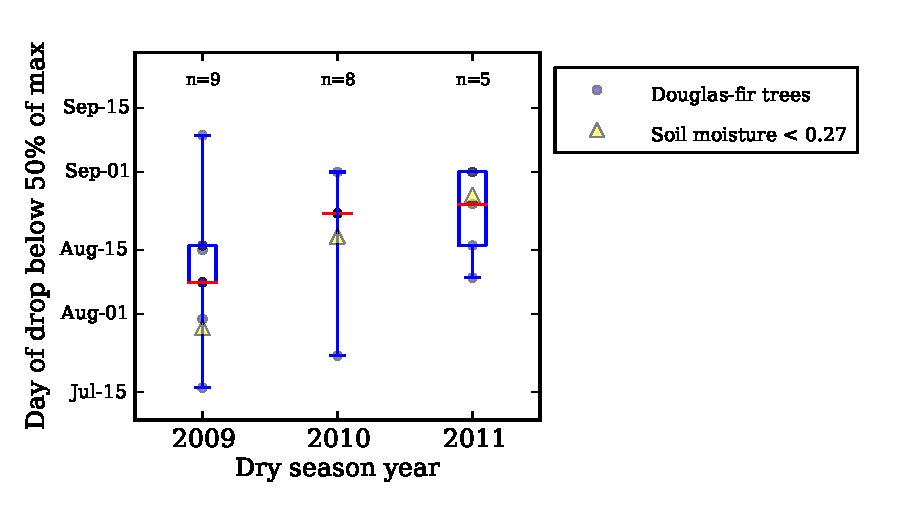
\includegraphics[width=0.9\textwidth]{ch1-sapflow/figures/Figure09.pdf}
\caption{Timing of dry season decline of Douglas-fir trees in each observation year. Each blue dot represents the date of decline below 50\% of a Douglas-fir tree's maximum daily integral, using only high VPD days (R3 daily max $>$2.5 kPa, linearly interpolating across gaps). The box diagram for each year shows the quartiles of the distribution of all Douglas-fir sensors, with the red line indicating the median. The yellow triangles show the date that site-averaged relative $\theta$ declined below 0.27.}
\label{fig:sapflow_interannual}
\end{figure}

The timing of onset of Douglas-firs' dry season decline varies between years.  Figure \ref{fig:sapflow_interannual} shows the date in each dry season when each Douglas-fir sensor dropped below 50\% of its maximum daily integral, using only high \textit{VPD} days (R3 daily max $>$2.5 kPa, linearly interpolating across gaps), and the box diagrams show the quartiles of the distribution of all Douglas-fir sensors in each year.  The timing of the sap flow decline varies among the three years, occurring approximately two weeks earlier in 2009 than in 2010 or 2011.  The timing of soil moisture depletion also varies among the years, with depletion happening earliest in 2009 and latest in 2011 (yellow triangles in Figure \ref{fig:sapflow_interannual}), largely due to the timing of the last spring storm.  The date of relative soil moisture decline below 0.27 and the median date of Douglas-fir decline below 50\% are close in all three years, although there is notable scatter.

\subsection{Regional transpiration estimates}

\begin{figure}[here]
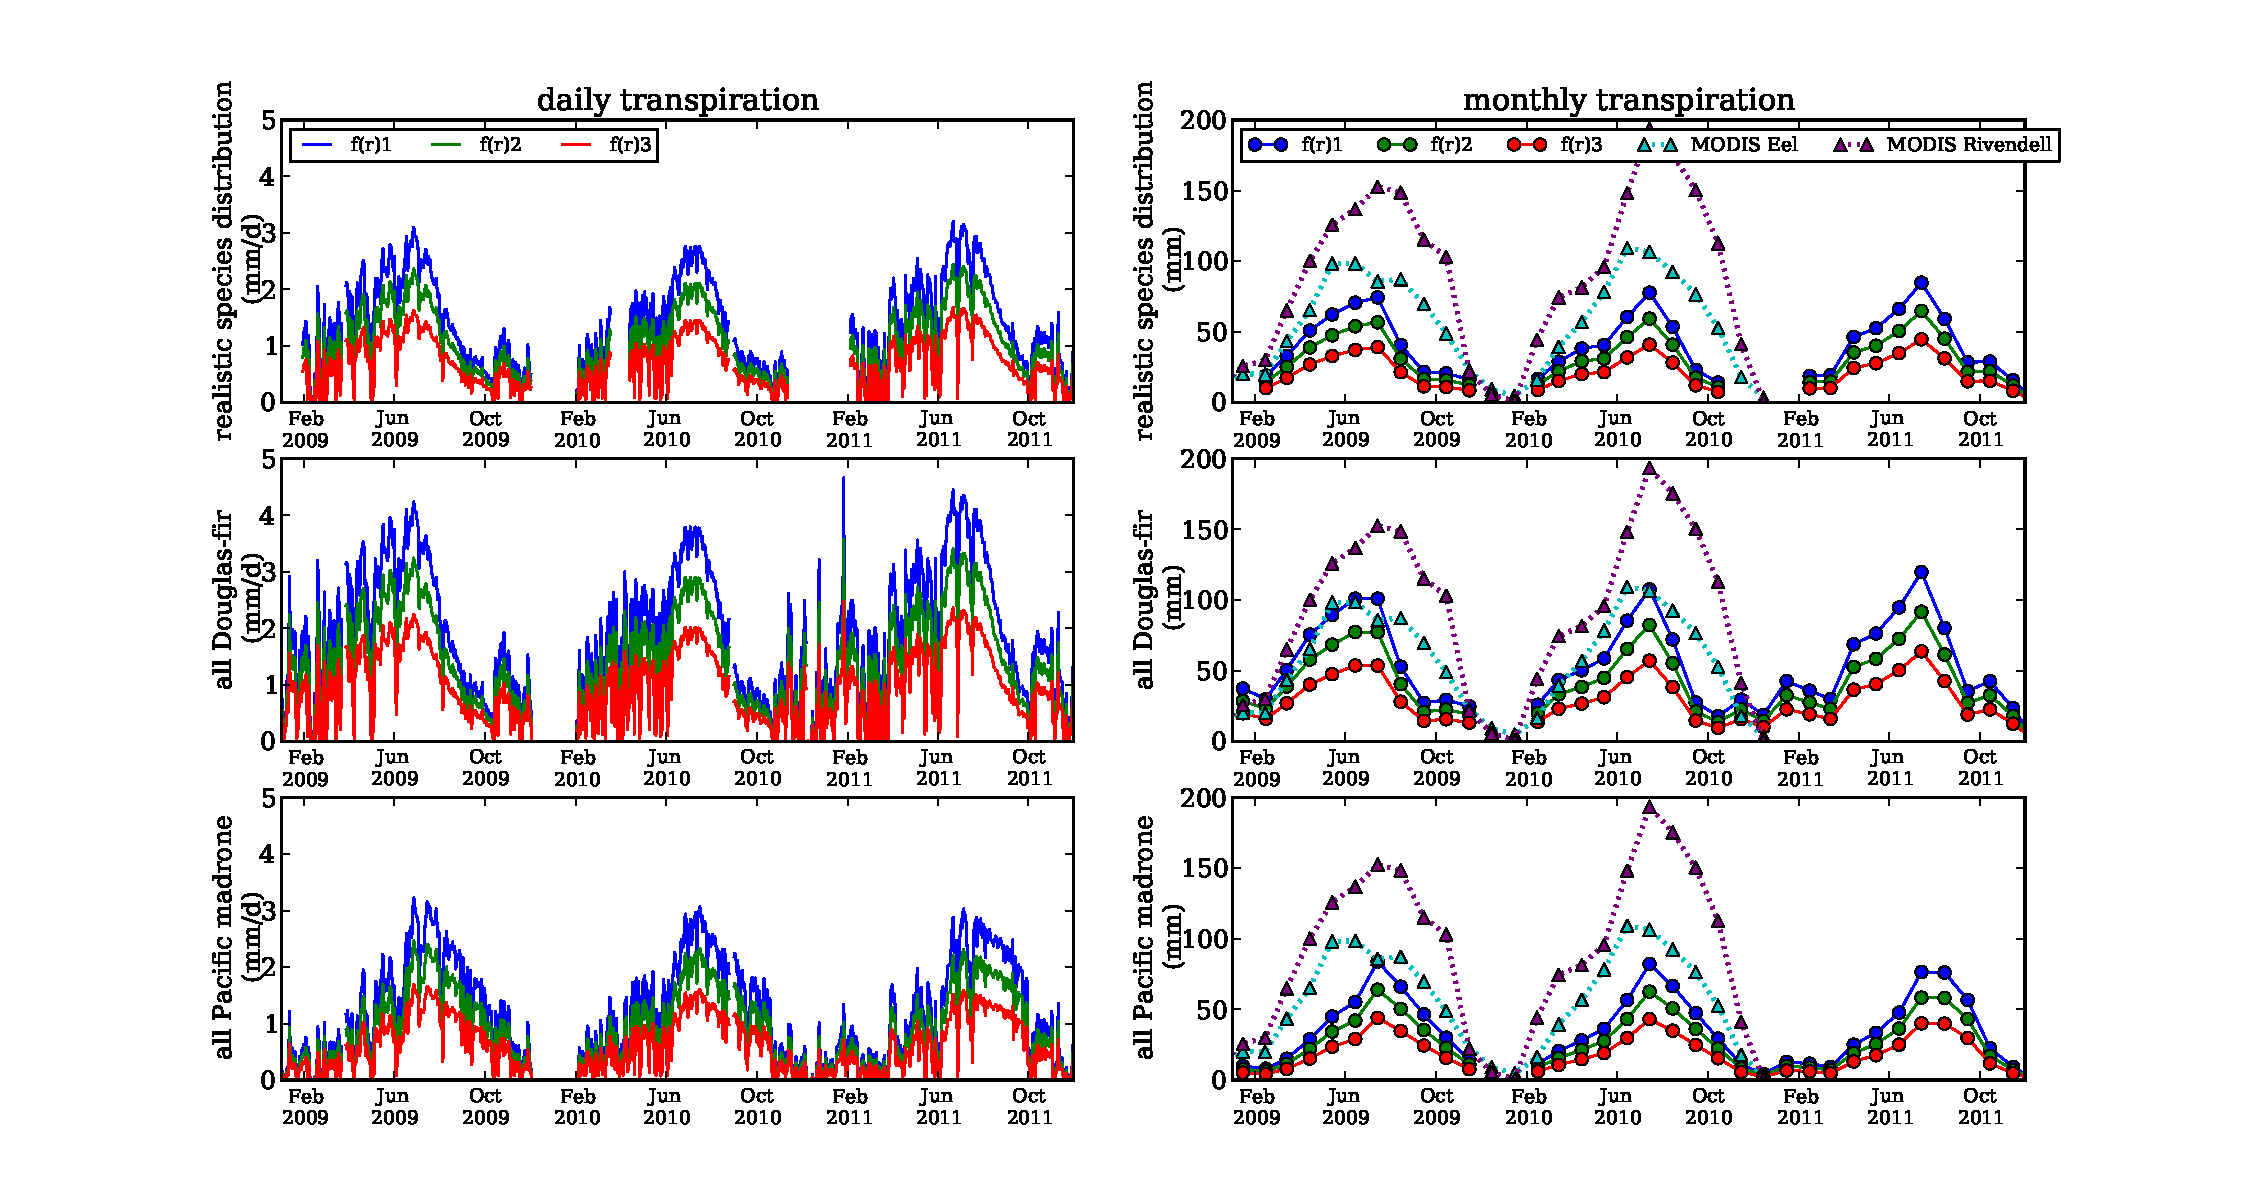
\includegraphics[width=0.9\textwidth]{ch1-sapflow/figures/Figure10.pdf}
\caption{Estimates of regional transpiration.  Left column: daily average transpiration rate estimated for the three plausible radial functions of sap velocity, using a realistic species distribution (top), assuming all trees are Douglas-fir (center), and assuming all trees are Pacific madrone (bottom.)  Right column: monthly integrals of transpiration estimates, again for the three plausible radial velocity profiles, and for the same three cases of species distribution.  Also shown in the right column are remote sensing estimates of monthly ET at two spatial scales: nearest MODIS pixel to the field site (purple), and MODIS estimate averaged over the Eel River watershed (cyan.)}
\label{fig:sapflow_regional}
\end{figure}

Our bottom-up estimates of regional transpiration, estimated with the aid of the FIA data, are shown at daily and monthly timescales in Figure \ref{fig:sapflow_regional} and are compared with a top-down remote sensing estimate of ET derived from MODIS through 2010 in Figure \ref{fig:sapflow_regional}, right column.  Our estimates using a realistic species distribution (row 1) show highest transpiration in June and July and a marked decline in the dry season.  The hypothetical all-Douglas-fir estimate (row 2) is very similar, which is not surprising because a large fraction of trees in the Eel watershed are Douglas-firs, redwoods, or other conifers, and thus the estimate in row 1 is strongly influenced by the Douglas-fir dynamics.  The all-Pacific-madrone hypothetical case (row 3), in contrast, has lower spring (February-May) transpiration and higher dry season (August and September) transpiration than either the realistic species distribution estimate or the all-Douglas-fir estimate.

The three radial sap velocity profiles tested give transpiration estimates that vary by approximately a factor of two.  The upper end of the range is similar in magnitude to the average of MODIS-derived ET for pixels in the Eel watershed (cyan in Figure \ref{fig:sapflow_regional}, right column.)  The sap-flow-based estimates are smaller than the MODIS-derived estimate of ET for the pixel nearest the Rivendell site (purple in Figure \ref{fig:sapflow_regional}, right column) by a factor of 2 to 3.

\begin{figure}[here]
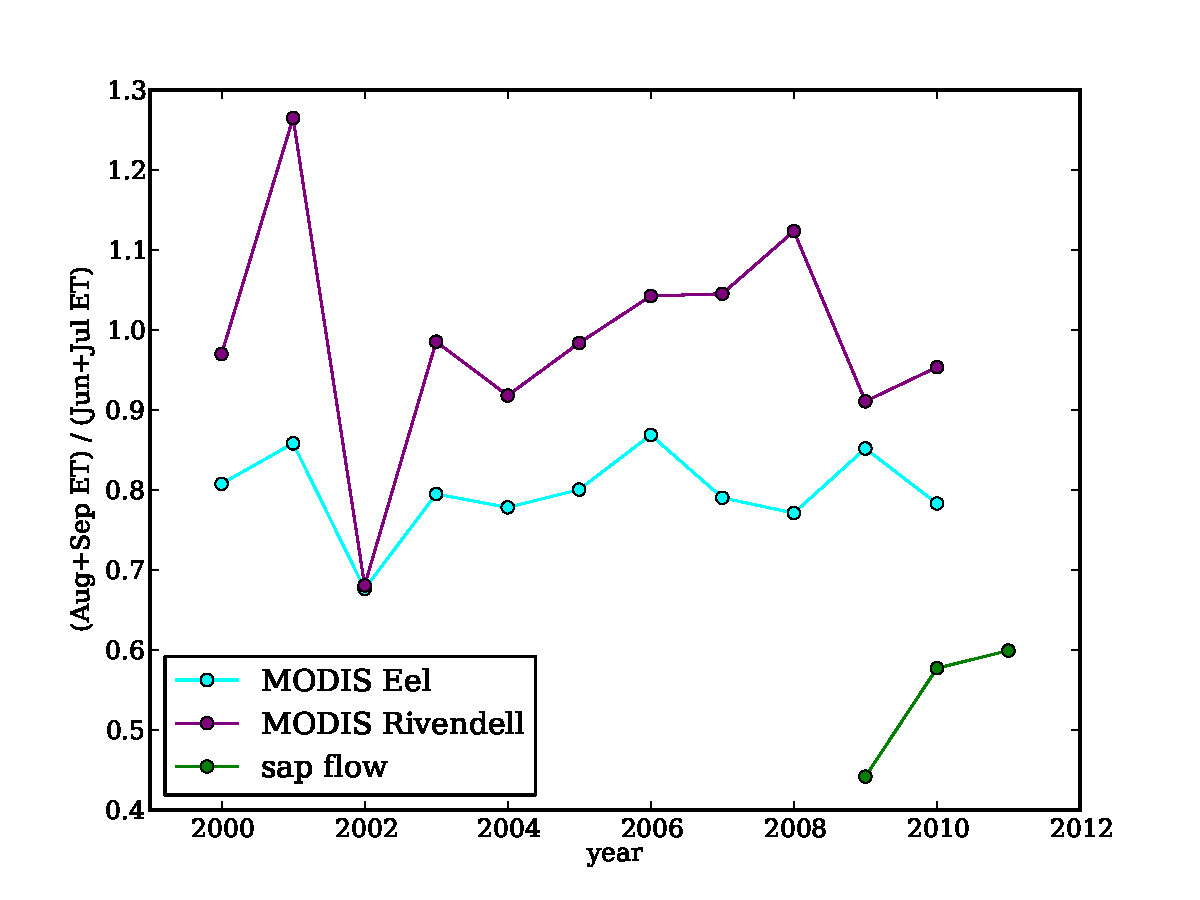
\includegraphics[width=0.9\textwidth]{ch1-sapflow/figures/Figure11.pdf}
\caption{Ratio of dry season to peak season ET (MODIS) or transpiration (sap flow); dry season is defined as August + September, and peak season is defined as June + July.  Two spatial scales are shown for MODIS: the pixel nearest to the Rivendell site (purple) and the average for all pixels in the Eel watershed (cyan.)}
\label{fig:sapflow_ratio}
\end{figure}

With the realistic species distribution, we estimate lower dry season (August-September) transpiration relative to peak (June-July) transpiration than does MODIS.  Figure \ref{fig:sapflow_ratio} shows August plus September transpiration divided by June plus July transpiration for MODIS-derived ET from 2000 to 2010, and for our estimates from 2009 to 2011.  In our estimates, the ratio of dry season transpiration to peak transpiration is the same regardless of radial sap velocity profile (the integral factor in Equation \ref{eqn:transpreg} cancels), so only one sap-flow-based estimate is shown in Figure \ref{fig:sapflow_ratio}.  The MODIS ratio of dry season transpiration to peak transpiration is close to 0.8 for the Eel watershed average and close to 1 for the near-Rivendell pixel for all years and is markedly higher than the sap-flow-based ratio, which is close to 0.5 in all three years.


